\let\negmedspace\undefined
\let\negthickspace\undefined
\documentclass[journal]{IEEEtran}
\usepackage[a5paper, margin=10mm, onecolumn]{geometry}
%\usepackage{lmodern} % Ensure lmodern is loaded for pdflatex
\usepackage{tfrupee} % Include tfrupee package

\setlength{\headheight}{1cm} % Set the height of the header box
\setlength{\headsep}{0mm}     % Set the distance between the header box and the top of the text

\usepackage{gvv-book}
\usepackage{gvv}
\usepackage{cite}
\usepackage{amsmath,amssymb,amsfonts,amsthm}
\usepackage{algorithmic}
\usepackage{graphicx}
\usepackage{textcomp}
\usepackage{xcolor}
\usepackage{txfonts}
\usepackage{listings}
\usepackage{enumitem}
\usepackage{mathtools}
\usepackage{gensymb}
\usepackage{comment}
\usepackage[breaklinks=true]{hyperref}
\usepackage{tkz-euclide} 
\usepackage{listings}
% \usepackage{gvv}                                        
\def\inputGnumericTable{}                                 
\usepackage[latin1]{inputenc}                                
\usepackage{color}                                            
\usepackage{array}                                            
\usepackage{longtable}                                       
\usepackage{calc}                                             
\usepackage{multirow}                                         
\usepackage{hhline}                                           
\usepackage{ifthen}                                           
\usepackage{lscape}
\begin{document}

\bibliographystyle{IEEEtran}
\vspace{3cm}

\title{1-1.11-5}
\author{EE24BTECH11064 - Harshil Rathan }
% \maketitle
% \newpage
% \bigskip
{\let\newpage\relax\maketitle}

\renewcommand{\thefigure}{\theenumi}
\renewcommand{\thetable}{\theenumi}
\setlength{\intextsep}{10pt} % Space between text and floats


\numberwithin{equation}{enumi}
\numberwithin{figure}{enumi}
\renewcommand{\thetable}{\theenumi}
\textbf{Question}:\\
The scalar product of the vector $\hat{\vec{a}}=\hat{i}+\hat{j}+\hat{k}$ with a unit vector along the sum of the vectors $\hat{\vec{b}}=2\hat{i}+4\hat{j}-5\hat{k}$ and $\hat{\vec{c}}=\lambda\hat{i}+2\hat{j}+3\hat{k}$ is equal to 1. Find the value of $\lambda$ and hence find the unit vector along $\hat{\vec{b}}+\hat{\vec{c}}$.
\\
\solution 
\begin{table}[h!]
    \centering
    \begin{tabular}[12pt]{ |c| c|}
    \hline
    \textbf{Equations}& \textbf{Given}\\ 
    \hline
     $2y$ & $3x+12$ \\
    \hline 
     $x$ & $2, 8 $\\
    \hline
    \end{tabular}
    \caption{Given Equations}

\end{table}
Find Sum,
\begin{align}
     \hat{\vec{b}}+\hat{\vec{c}}= (2\hat{i}+4\hat{j}-5\hat{k})+(\lambda\hat{i}+2\hat{j}+3\hat{k})
\end{align}    
\begin{align}    
\hat{\vec{b}}+\hat{\vec{c}}=(2+\lambda)\hat{i}+6\hat{j}-2\hat{k}
\end{align}
Find Magnitude,
\begin{align}
\|\hat{\vec{b}}+\hat{\vec{c}}\|=\sqrt{(2+\lambda)^2+6^2+(-2)^2}
\end{align}
\begin{align}
\|\hat{\vec{b}}+\hat{\vec{c}}\|=\sqrt{(2+\lambda)^2+40}
\end{align}
Unit vector $\hat{\vec{u}}$ in direction of $\hat{\vec{b}}+\hat{\vec{c}}$ is,
\begin{align}
\hat{\vec{u}}=\frac{\hat{\vec{b}}+\hat{\vec{c}}}{\|\hat{\vec{b}}+\hat{\vec{c}}\|}
\end{align}
Scalar Product with $\hat{\vec{a}}$
\begin{align}
    \hat{\vec{a}} \cdot \hat{\vec{u}} =1\\
    \hat{\vec{a}} \cdot \frac{\hat{\vec{b}}+\hat{\vec{c}}}{\|\hat{\vec{b}}+\hat{\vec{c}}\|} =1
\end{align}
\begin{align}
    \hat{\vec{a}} \cdot (\hat{\vec{b}+\vec{c}})=\|\hat{\vec{b}}+\hat{\vec{c}}\|
\end{align}
\begin{align}
    (\hat{i}+\hat{j}+\hat{k}) \cdot (2+\lambda)\hat{i}+6\hat{j}-2\hat{k}=\|\hat{\vec{b}}+\hat{\vec{c}}\|
\end{align}
\begin{align}
    \lambda+6=\|\hat{\vec{b}}+\hat{\vec{c}}\|
\end{align}
\begin{align}
    \lambda+6=\sqrt{(2+\lambda)^2+40}
\end{align}
On solving,
\begin{align}
    \lambda=1
\end{align}
Unit Vector $\hat{\vec{u}}$ is,
\begin{align}
    \hat{\vec{u}}=\frac{3\hat{i}+6\hat{j}-2\hat{k}}{7}\\
     \hat{\vec{u}}=\frac{3\hat{i}}{7}+\frac{6\hat{j}}{7}-\frac{2\hat{k}}{7}
\end{align}
Therefore
\begin{align}
    x=\frac{3}{7},y=\frac{6}{7},z=\frac{-2}{7}
\end{align}
\begin{figure}[h!]
   \centering
   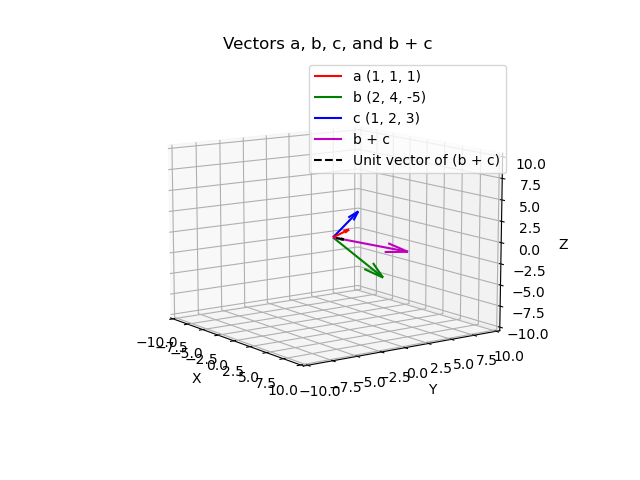
\includegraphics[width=\linewidth]{figs/Figure_1.png}
   \caption{}
   \label{stemplot}
\end{figure}





\end{document}
